\documentclass[letter,11pt]{article}

\usepackage{amsfonts}
\usepackage{amsmath}
\usepackage{amssymb}
\usepackage[brazilian]{babel}
\usepackage{enumerate}
\usepackage[T1]{fontenc}
%\usepackage[ansinew,latin1]{inputenc}
\usepackage[utf8x]{inputenc}
\usepackage{multicol}
\usepackage{graphicx}
\setlength\columnseprule{0.5pt}
\newtheorem{exer}{Exercício}

\newcommand{\var}{Var}
\newcommand{\E}{\mathbb{E}}

\newcommand{\mat}[1]{\mbox{\boldmath{$#1$}}}

\usepackage[letterpaper,top=3cm, bottom=2cm, left=2.5cm, right=2.5cm]{geometry}

\begin{document}

%\thispagestyle{empty}
\begin{center}{ \Large MAT02023 - Inferência A }\end{center}

\begin{center}
{\large  \sc Gabarito Lista 1 - Revisão}
\end{center}
\vspace{15mm}


\noindent \textit{\textbf{Matemática elementar}} \\
\noindent \textbf{Exercícios 1 ao 8}

\includegraphics[scale=0.4]{2017-05-15-PHOTO-00000032}

\includegraphics[scale=0.4]{2017-05-15-PHOTO-00000033}


\newpage
\bigskip
\noindent \textit{\textbf{Introdução à Probabilidade}}

\medskip
\setcounter{exer}{8}
\medskip
\begin{exer} \rm %Livro pg 63

\begin{enumerate}[a)]
\item R: 1/21
\item  R: 3/7
\item  R: 91/21 
\item  R:  $\frac{441}{21}-\left(\frac{91}{21}\right)^2=2.22$
\end{enumerate}
\end{exer}





\medskip
\begin{exer} \rm
\begin{enumerate}[a)]

\item  $a=3/14$ e $b=1/14$ 
\item 27/14

\item 2.21

\item  8.84

\end{enumerate}
\end{exer}






\medskip
\begin{exer} \rm %Material Lisi
R: P(X=0)=0.5, P(X=1)=0.35, P(X=2)=0.12 P(X<3)=0.5+0.35+0.12=0.9659
\end{exer}




\medskip
\begin{exer} \rm %livro
 R: 0.665, 0.619 e 0.597 aproximadamente.
\end{exer}


\medskip
\begin{exer} \rm %livro

\begin{enumerate}[a)]
\item R: $\frac{81}{128}$
\item R: $\frac{819}{1982}$
\end{enumerate}
\end{exer}



\medskip
\begin{exer}\rm 
Denote $\hat{p}$ a proporção estimada de ratos que desenvolvem um certo tipo de tumor quando submetidos a radiação. Assumindo que $X_1, \ldots, X_n$ são i.i.d. segundo $X \sim Bernoulli(p)$, então sabemos que $Y = \sum_{i=1}^{n} X_i \sim Binomial(n,p)$. Por consequência 
$$E(\hat{p}) = n^{-1} E \left( Y \right) = p$$
e
$$Var(\hat{p}) = n^{-2} Var \left( Y \right) = n^{-1} p (1-p).$$

\noindent $P \left( \left| \hat{p} - p \right| < 0,02 \right) = P \left( -0,02 < \hat{p} - E(\hat{p}) < 0,02 \right) = P \left( \frac{-0,02}{\sqrt{Var(\hat{p})}} < \frac{\hat{p} - E(\hat{p})}{\sqrt{Var(\hat{p})}} < \frac{0,02}{\sqrt{Var(\hat{p})}} \right) \geq 0.9$. 

Assumindo que as condições do CLT valem para $\hat{p}$ temos $Z = \frac{\hat{p} - E(\hat{p})}{\sqrt{Var(\hat{p})}} \sim Normal(0,1)$ e que $P(Z < 1,64) \geq 0.95$. Então, para satisfazer a condição acima
$ P \left( Z < \frac{0,02}{\sqrt{Var(\hat{p})}} \right) \geq 0.95$, portanto
$$ \frac{0,02}{\sqrt{Var(\hat{p})}} = 1,64 \Leftrightarrow \frac{0,02}{\sqrt{n^{-1} p (1-p)}} = 1,64 \Leftrightarrow n = \frac{1,64^2 \times p \times (1-p)}{\sqrt{0,02^2}}.$$

\begin{enumerate}[a)]
\item Na falta de informação sobre o verdadeiro valor de $p$, se usarmos $p=0,5$ nos dará o maior tamanho de amostra
e $n = 1681$.
\item Usando $p=0,2$ teremos $n=1076$.
\end{enumerate}
\end{exer}
 
 
 
 
 
 \medskip
\begin{exer}\rm 
Sim. 865 indiv?duos. 
\end{exer}




\medskip
\begin{exer} \rm
\begin{enumerate}[a)]
\item  R. $\alpha=3$
\item  R. $\alpha=5/4$. 
\end{enumerate}
\end{exer} %Material Lisi



\medskip
\begin{exer} \rm
\begin{enumerate}[a)]
\item R: 2
\item R: 1/4
\item R: $F(x)=\begin{cases} 1-x^{-2},\quad \mbox{ se } x\geq 1\\
                       0, \quad \quad       \mbox{ se } x<1.
        \end{cases}$
\end{enumerate}
\end{exer}%livro 





\medskip
\begin{exer} \rm
\begin{enumerate}[a)]
\item R:$P(X>1200)=0,3012$
\item R: média=1000;   $P(X<1000)=0,6321$
\item R:  x=693,15
\end{enumerate}
\end{exer}


\medskip
\begin{exer} \rm 
\begin{enumerate}[a)]
\item R:  $X \sim Exp(1)$
            
   $P(X<0,25)=0,2212$

\item R: $P(X>0,75)=0,4724$
\end{enumerate}
\end{exer}






\medskip
\begin{exer} \rm R: P(X<1)=0,3297
\end{exer}




\medskip
\begin{exer} \rm
R: 0,1085
\end{exer}%livro




\medskip
\begin{exer} \rm R: $E(L)=3.980,59$
\end{exer}



\medskip
\begin{exer} \rm R: 73,19 	nota máxima para receber conceito A

70,33	nota máxima para receber conceito R
\end{exer}




\medskip
\begin{exer} \rm
Utilize o R para:
\begin{enumerate}[a)]
  \item 
  \begin{verbatim}
## Poisson case
# set up
lambda <- 5                 # parametro
n <- 10                     # tamanho da amostra
xgen <- rpois(n, lambda)    # amostra gerada
  \end{verbatim}
  \item 
  \begin{verbatim}
dfgen <- data.frame(xgen)
# empirical cdf plot  
plotecdf <- ggplot(dfgen, aes(xgen)) + 
            stat_ecdf(colour="red", alpha = 0.5) + 
            labs(title="Empirical Cumulative \n Distribution Function", 
                 y = expression(F[x]), x = "x")
plotecdf
  \end{verbatim}
  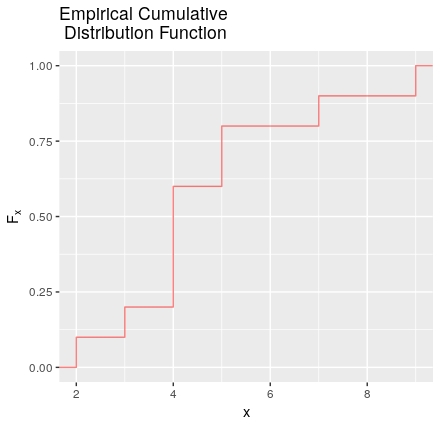
\includegraphics[scale=0.5]{exe_ecdf1}
  
  \item 
    \begin{verbatim}
# plot multiple samples with fixed n
n <- 10
nsim <- 10
lambda <- 5
xgen <- rpois(n * nsim, lambda)
dfgen <- data.frame(xgen, g = factor(rep(1:nsim, rep(n, nsim))))
plotfixedn <- ggplot() 
for(i in 1:nsim){
  # print(plotfixedn + stat_ecdf(aes(xgen), dfgen, colour = "red", alpha = 0.5))
  plotfixedn <- plotfixedn + stat_ecdf(aes(xgen), dfgen[dfgen$g==i,], 
                                       colour = "red", alpha = 0.2)
}
plotfixedn + labs(title=paste("Cumulative Distribution Function \n", nsim, 
                              " samples of size ",n), y = expression(F[x]), 
                  x = "x")
  \end{verbatim}
  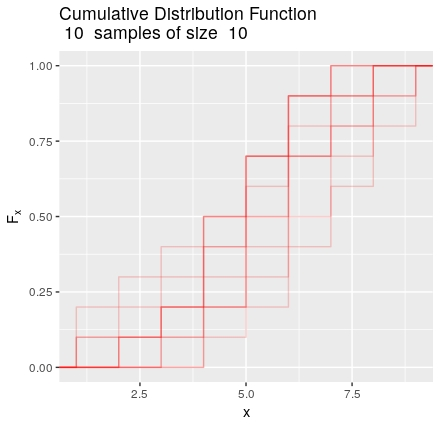
\includegraphics[scale=0.5]{exe_ecdf2}
  
  \item 
  \begin{verbatim}
# funcao para calfular Fn(x) de 'nsim' amostras geradas de tamanho 'n'
Fnx <- function(n, x, nsim){
  # n    - tamanho da amostra
  # x    - particular valor da Poisson
  # nsim - número de simulacoes
  
  Fnxgen <- NULL                # objeto para guardar os Fn(x)'s
  for(i in 1:nsim){
    xgen <- rpois(n, lambda)    # gera amostra
    Fn <- ecdf(xgen)            # calcula CDF
    Fnxgen <- c(Fnxgen, Fn(5))   # armazena Fn(x)
  }
  hist(Fnxgen, main=paste("tamanho amostra n =", n), xlab=paste("Fn(",x,")"))
  abline(v=ppois(5, lambda), col="red")     # F(x) real
}
par(mfrow=c(2,2))
Fnx(10, 5, 100)
Fnx(100, 5, 100)
Fnx(1000, 5, 100)
Fnx(10000, 5, 100)
  \end{verbatim}
  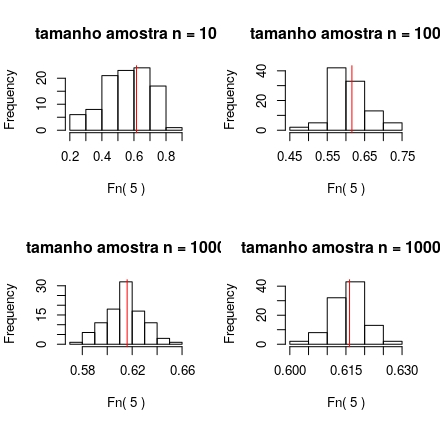
\includegraphics[scale=0.5]{exe_ecdf3}
\end{enumerate}
\end{exer}
  
\end{document}